\subsection*{Epidemiologia e Redes Complexas}
Na epidemiologia, a análise de redes tem se mostrado uma abordagem fundamental para estudar a transmissão de doenças infecciosas e entender a estrutura dos contatos entre indivíduos infectados. Dentre as diversas contribuições nesse campo, destaca-se o livro "Mathematics of Epidemics on Networks" \cite[]{2017_Kiss_BOOK}, que explora a aplicação do modelo SIR (Susceptível-Infectado-Recuperado) em redes complexas, em que os nós representam indivíduos e as arestas representam as interações entre eles. O livro desvenda como a estrutura da rede pode influenciar a propagação de doenças, investigando questões como o papel dos nós centrais na disseminação das enfermidades, a eficácia de diferentes estratégias de controle e intervenções, bem como o impacto de características topológicas específicas na dinâmica das epidemias. Uma das contribuições centrais do livro é a introdução do conceito de estrutura de redes em formato de gravata borboleta, a qual permite uma análise mais profunda e abrangente das redes complexas.
Essa estrutura é composta por três principais componentes: a Área Central (SCC), a Seção de Entrada (IN) e a Seção de Saída (OUT). Matematicamente, podemos representar esses componentes de acordo com o seguinte modelo:

\begin{equation}
	\text{{SCC}} = { v \in V : \forall u,w \in \text{{SCC}}, \text{{existe um caminho direto de }} u \text{{ para }} w }
\end{equation}

\begin{equation}
	\text{{IN}} = { v \in V : \exists u \in \text{{SCC}}, \text{{ tal que }} (u,v) \in E \text{{ e não existe um caminho direto de }} v \text{{ para }} u }
\end{equation}

\begin{equation}
	\text{{OUT}} = { v \in V : \exists u \in \text{{SCC}}, \text{{ tal que }} (v,u) \in E \text{{ e não existe um caminho direto de }} u \text{{ para }} v }
\end{equation}

Onde $V$\simbolo{V}{Representa um conjunto de nós em um grafo} representa o conjunto de nós e $E$\simbolo{E}{Representa um conjunto de arestas em um grafo} o conjunto de arestas da rede. A Área Central {SCC} consiste em nós altamente conectados, em que há um caminho direto de um nó para qualquer outro nó da área central. A Seção de Entrada {IN} é composta por nós que possuem conexões direcionadas para a área central, mas não têm caminhos de retorno diretos para os nós da Seção de Saída {OUT} ou da área central. Analogamente, a Seção de Saída {OUT} inclui nós que têm conexões direcionadas da área central, mas não possuem caminhos de retorno diretos para os nós da Seção de Entrada {IN} ou da área central.

Essa estrutura de redes em formato de gravata borboleta tem o potencial de ser aplicada para interpretar grafos direcionados em redes sociais. Ao analisar uma rede social, podemos identificar a Área Central {SCC} como os indivíduos ou grupos altamente conectados que desempenham um papel central na propagação de informações ou influência na rede. A Seção de Entrada {IN} representa os nós que interagem com a Área Central, mas não possuem conexões diretas entre si. Esses nós podem desempenhar um papel crucial ao receber informações da Área Central e disseminá-las para outros nós da rede. Da mesma forma, a Seção de Saída {OUT} inclui os nós que têm conexões direcionadas para a Área Central, mas não estão diretamente conectados uns aos outros. Esses nós podem ser responsáveis por disseminar informações ou influência da Área Central para outras partes da rede.

A propagação de fake news em redes sociais pode ser comparada à disseminação de doenças infecciosas, em que a informação falsa se espalha de maneira semelhante a um contágio. A estrutura de redes em formato de gravata borboleta, descrita no livro, pode ajudar a identificar os nós centrais e influentes que desempenham um papel importante na disseminação de informações falsas. Além disso, a análise da dinâmica da propagação de fake news pode se beneficiar das técnicas e modelos matemáticos discutidos no livro para compreender a rapidez e o alcance dessa disseminação.

Uma outra contribuição importante é na epidemiologia não Markoviana. Os modelos estocásticos de epidemias não markovianas (Stochastic non-Markovian epidemics) são uma extensão dos modelos clássicos de epidemias, que consideram a dependência temporal e complexa das interações entre os eventos em um processo epidêmico. Esses modelos reconhecem que a probabilidade de transição entre estados pode depender do histórico completo de estados anteriores, levando em conta fatores como a história de exposição, imunidade adquirida e comportamentos individuais. Matematicamente, podemos representar um modelo estocástico de epidemia não markoviana como:

\begin{equation}
	P(S(t+\Delta t), I(t+\Delta t), R(t+\Delta t)|S(t), I(t), R(t), \mathcal{H}(t))
\end{equation}

onde $S(t)$, $I(t)$ e $R(t)$ representam o número de indivíduos suscetíveis, infectados e recuperados no tempo $t$, respectivamente, e $\mathcal{H}(t)$ denota o histórico completo dos eventos até o tempo $t$.

A aplicação dos modelos estocásticos de epidemias não markovianas na análise de redes sociais pode fornecer insights importantes para entender fenômenos como polarização e câmaras de eco. Ao considerar a dependência temporal nas interações sociais, esses modelos podem capturar como a exposição a determinadas opiniões ou informações no passado influencia a propensão de um indivíduo em adotar ou compartilhar essas opiniões no futuro. Essa dependência temporal pode ser representada por meio de uma função de probabilidade condicional:

\begin{equation}
	P(I(t+\Delta t)|I(t), \mathcal{H}(t))
\end{equation}

Essa abordagem permite investigar como a formação e a propagação de polarização e câmaras de eco ocorrem ao longo do tempo em uma rede social. Por exemplo, pode-se analisar como a exposição a opiniões semelhantes influencia a adesão a um grupo específico e a formação de câmaras de eco, onde informações são amplificadas e reforçadas dentro de determinados grupos, resultando em uma maior polarização entre eles. Além disso, a aplicação desses modelos permite explorar o papel dos nós centrais na disseminação de polarização, bem como o impacto de intervenções e estratégias de controle na quebra das câmaras de eco e na redução da polarização.

Dessa forma, a utilização de modelos estocásticos de epidemias não markovianas na análise de redes sociais oferece uma abordagem poderosa para investigar e compreender os mecanismos subjacentes à formação de polarização e câmaras de eco. A inclusão da dependência temporal e das interações complexas entre os indivíduos permite uma representação mais realista dos processos sociais em redes complexas, proporcionando insights valiosos para o desenvolvimento de estratégias de mitigação e intervenções eficazes no combate à polarização e à formação de câmaras de eco em redes sociais.

A integração de eventos estocásticos, no contexto das redes sociais, pode ser relacionada aos momentos de grande tráfego ou atividade intensa nessas plataformas. Esses eventos podem ser caracterizados por um aumento significativo no número de interações, compartilhamentos, curtidas e comentários em determinados conteúdos. Matematicamente, podemos representar esses eventos estocásticos como:

\begin{equation}
	P(S(t+\Delta t), I(t+\Delta t), R(t+\Delta t)|S(t), I(t), R(t), \mathcal{H}(t), \mathcal{T}(t))
\end{equation}

onde $\mathcal{T}(t)$ denota o histórico completo dos eventos de tráfego e atividade na rede social até o tempo $t$.

A introdução de hashtags como dados de entrada nessa análise pode ser feita considerando-as como fatores de disseminação de informações análogos ao contágio na epidemiologia clássica. A presença e popularidade de uma hashtag específica podem influenciar a propagação de informações relacionadas a um determinado tópico na rede social. Isso pode ser representado matematicamente pela função de probabilidade condicional:

\begin{equation}
	P(I(t+\Delta t)|I(t), \mathcal{H}(t), \mathcal{T}(t), \mathcal{C}(t))
\end{equation}

onde $\mathcal{C}(t)$ representa o conjunto de hashtags relevantes e populares até o tempo $t$.

A inclusão das hashtags nessa análise permite uma compreensão mais abrangente e precisa da disseminação de informações nas redes sociais. Elas atuam como marcadores temáticos e podem desempenhar um papel importante na formação de comunidades online, na viralização de conteúdos específicos e na amplificação de certas mensagens. As hashtags funcionam como vetores de contágio, direcionando a atenção dos usuários para tópicos específicos e influenciando a propagação de informações relacionadas.

Ao incorporar as hashtags como fator de disseminação de informação na análise estocástica de redes sociais, é possível investigar como sua presença e popularidade influenciam a adesão dos usuários a determinados tópicos, a propagação de informações e a formação de comunidades temáticas. A análise da dependência temporal e da interação complexa entre as hashtags e o histórico de eventos na rede social pode fornecer insights valiosos sobre a dinâmica da disseminação de informações e ajudar a identificar padrões de comportamento e tendências emergentes.

Em resumo, a integração de eventos estocásticos no contexto das redes sociais, juntamente com a consideração das hashtags como fator de disseminação de informação análoga ao contágio na epidemiologia clássica, permite uma análise mais abrangente e precisa da propagação de informações e da formação de comunidades temáticas. Essa abordagem contribui para a compreensão dos processos sociais em redes complexas, fornecendo insights valiosos para a identificação de tendências, a criação de estratégias de engajamento e o desenvolvimento de intervenções eficazes na disseminação de informações em redes sociais.

\citeonline{2005_Christley} utilizaram a análise de redes para entender como a gripe se espalha em uma população, o que pode ajudar a desenvolver estratégias de prevenção mais eficazes.
\begin{figure}[!htb]
	\caption{Ilustração esquemática de uma topologia em formato de gravata borboleta}
	\label{fig:network_bowtie}
	\centering
	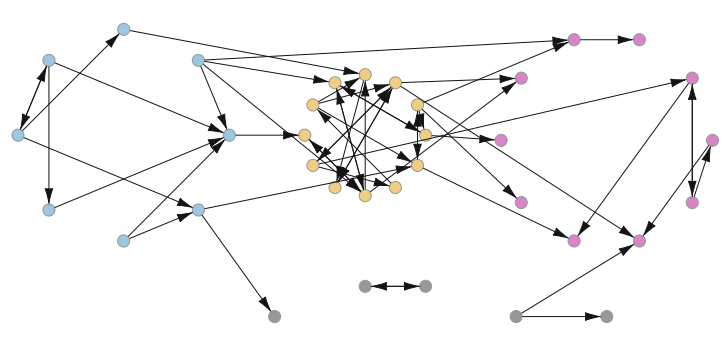
\includegraphics[width=\textwidth]{network_bowtie.png}
	\fdireta{2017_Kiss_BOOK}
\end{figure}